
\section{Desarrollo de Hardware}
\subsection{Arquitectura Controlador de Vuelo}
\\
Durante la fase inicial del proyecto, se realizó una revisión bibliográfica para definir los componentes esenciales en un controlador de vuelo. Basándome en esta investigación, se diseñó un esquema general de la arquitectura que seguiría el controlador de vuelo, tal y como se muestra en la Figura \ref{fig:arqui_controlador}.\\ \\

La unidad de procesamiento en la arquitectura del controlador de vuelo está a cargo del microcontrolador \textbf{ESP32-S3}, que proporciona un procesamiento potente y una gran flexibilidad en la comunicación con otros componentes del sistema. Este microcontrolador de doble núcleo opera a una velocidad de hasta 240 MHz y cuenta con conectividad Wi-Fi y Bluetooth 5.0. Maneja la intercomunicación mediante diversos protocolos estandarizados como I2C, UART y SPI, permitiendo una interacción eficiente con múltiples dispositivos periféricos.\\ \\

Es relevante mencionar que, en la mayoría de las arquitecturas estudiadas, se utiliza el microcontrolador STM32 Nucleo F767ZI, que, aunque es una opción de alto desempeño con un núcleo ARM Cortex-M7 a 216 MHz, 32 bits, y varias interfaces de comunicación, no cuenta con las capacidades integradas de velocidad, Wi-Fi y Bluetooth que ofrece el ESP32-S3.\\ \\



Un aspecto crítico es que se incluyen dos Unidades de Medición Inercial \textbf{(IMUs)}, una actuando como primaria y la otra como secundaria o de respaldo. Este esquema de redundancia aumentará la fiabilidad del sistema. En caso de que falle una \textbf{IMU}, la otra puede tomar el control inmediatamente, y así continuar la recolección de datos sobre orientación y movimiento, que son parámetros críticos para la estabilidad y navegación del UAV.
\vspace{5 px}

Los \textbf{IMUs} a utilizar serán modelos de alta precisión que proporcionan datos esenciales para la orientación, aceleración y velocidades angulares, siendo estos necesarios para las operaciones de vuelo autónomo del UAV y la estabilización del vehículo.
\\
La Figura \ref{fig:arqui_controlador} muestra el diagrama de la arquitectura del controlador de vuelo propuesto, donde se pueden observar los diferentes componentes y su interconexión. Este diagrama destaca la disposición del \textbf{ESP32-S3} en el centro, gestionando la comunicación con los sensores, actuadores y unidades de almacenamiento a través de los protocolos \textbf{I2C}, \textbf{UART}, y \textbf{SPI}. La redundancia en las \textbf{IMUs} permite que se tenga un sistema de respaldo que pueda reorientar a la aeronave en un caso crítico (sistema de redundancia), lo que junto con la incorporación de sensores adicionales como el \textbf{GPS}, \textbf{Barómetro}, y el \textbf{sistema de almacenamiento} aseguran un sistema robusto y fiable.


\vspace{5 px}


\begin{figure}[H]
    \centering
    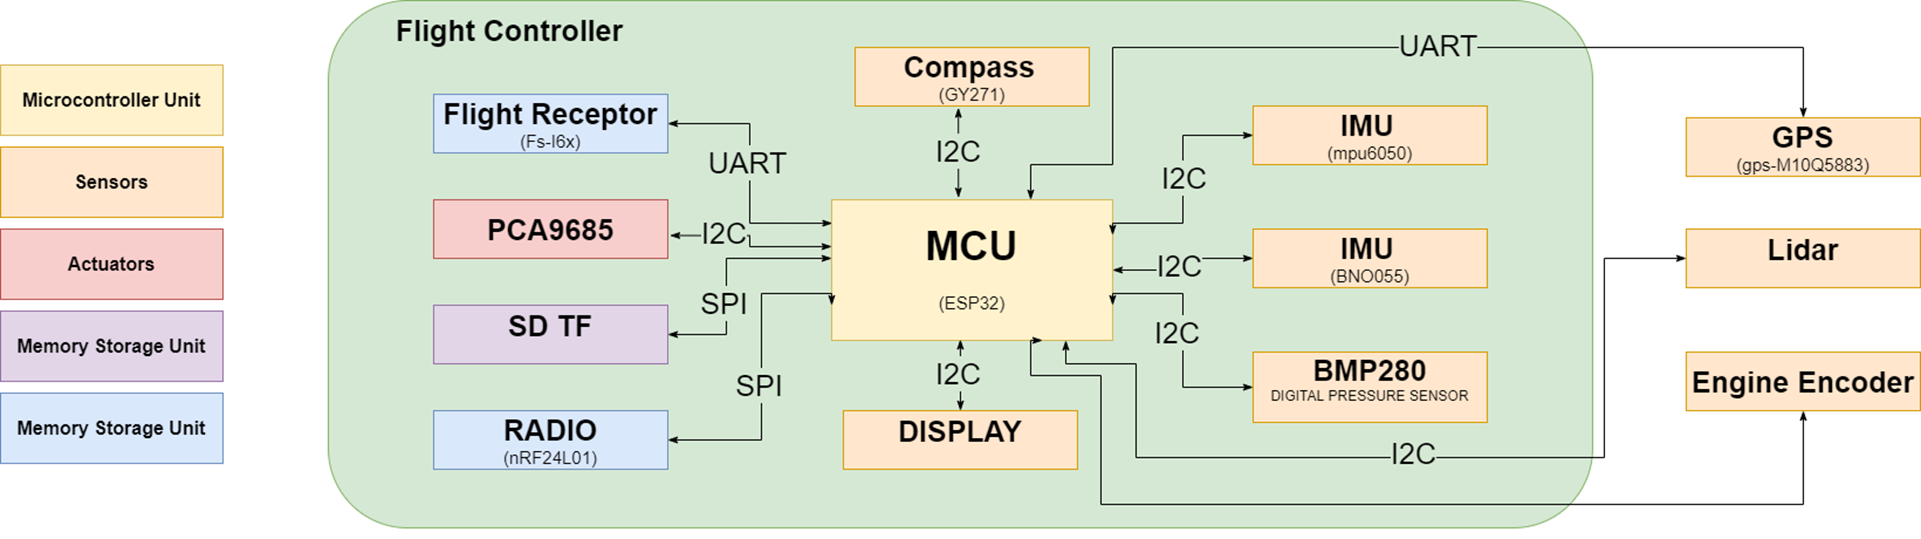
\includegraphics[width=\textwidth]{Imagenes/Metodologia/arquitectura_controlador.png}
    \caption{Arquitectura del controlador de vuelo diagrama de Caja Gris }
    \label{fig:arqui_controlador}
\end{figure}

Para ver de forma más detallada como sería esta arquitectura y como se integraría con los distintos módulos, se desarrollo el siguiente diagrama de Caja Blanca (véase \ref{fig:arqui_Blanxa}) , en el que se puede observar con más detalle cuales serán los componentes principales en la estructura del dispositivo. De este diagrama todos los dispositivos que están encapsulados por el recuadro verde, indican que están inmersos en el sistema mientras que todos los que se encuentran por fuera son módulos adicionales o que se encuentran en otra parte del Sistema.

\begin{figure}[H]
    \centering
    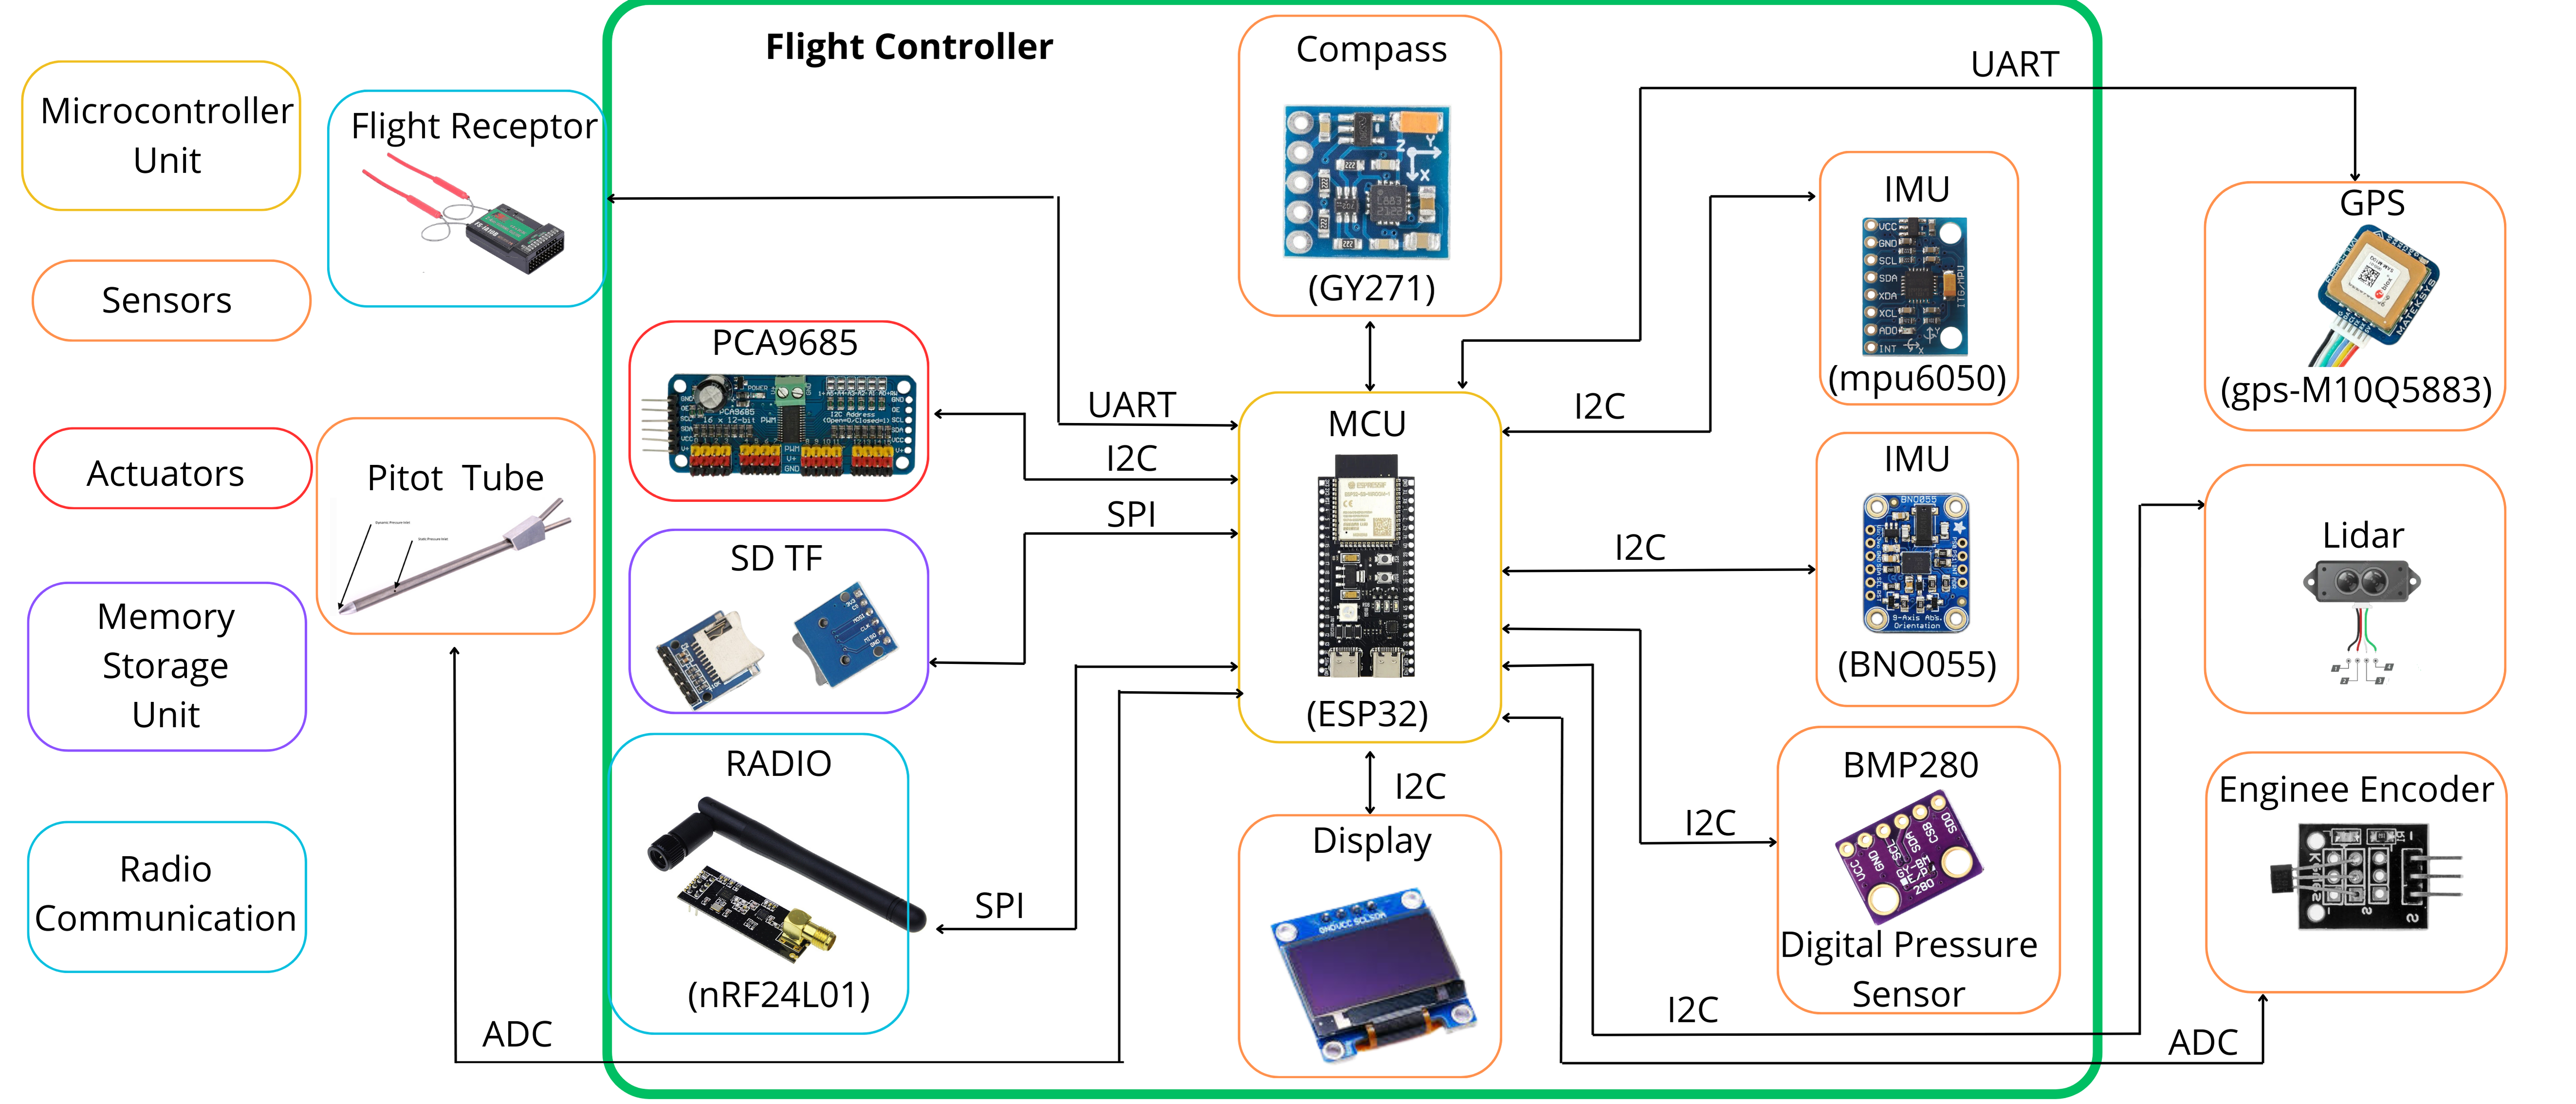
\includegraphics[width=\textwidth]{Imagenes/Metodologia/arquitecturaModulos.png}
    \caption{Arquitectura del controlador de vuelo diagrama de Caja Blanca }
    \label{fig:arqui_Blanxa}
\end{figure}

\subsection{Circuito Impreso}
Una vez finalizada la etapa de diseño y habiendo terminado de definir los componentes que conformaran el sistema, se procede a diseñar un circuito impreso \textbf{PCB}. A lo largo de este proyecto se realizaron en total 2 iteraciones del circuito para mejorar la estabilidad y eficiencia del circuito. El primer circuito fabricado se puede observar en \ref{fig:sch-1.0}, \ref{fig:pcb-1.0} y \ref{fig:pcb-ensambled-1.0}. Para esta primera iteración se utilizó como \textbf{MCU} un \textbf{ESP32 DevKit v1}, el cual presentaba ciertas deficiencias relacionadas con el protocolo I2C. En esta versión, el módulo \textbf{PCA9685} tenía un voltaje de alimentación lógico de \textbf{5V}, mientras que todos los demás voltajes de alimentación de los módulos de I2C se encontraban alimentados con \textbf{3.3V}. Esto generaba errores con los buses de \textbf{SDA} y \textbf{SCL}. Este error se puede abordar de dos formas. Agregando resistencias de \textbf{Pull-Up} de \textbf{4.7 k$\Omega$}, o alimentando toda la parte lógica a \textbf{3.3V}. Se decidió optar por la segunda opción. \\ \\
    


Otro problema relacionado con la \textbf{PCA9685} fue el de alimentación del pin \textbf{V+} o el voltaje de entrada del módulo. Puesto que inicialmente se tenía este dispositivo alimentado a una tensión de \textbf{+5v}, la cual al momento de realizar pruebas de movimiento de los servomotores generaba un consumo elevado de corriente que causaba un overshoot de voltaje y ocacionaba un reset en el dispositivo. 


\subsubsection{ Diseño del Esquemático Final}\\ \\

El software donde se diseñaron las dos versiones del circuito fue \textbf{KIcad} versión \textbf{8.0}. Este software fue seleccionado, puesto que es \textbf{Open Source} y hay un gran número de huellas y componentes creados por la comunidad. \\

Para el apartado de diseño del circuito impreso se hace necesario diseñar el esquemático a seguir, el cual consiste en la selección y asociación de \textbf{símbolos} y \textbf{huellas} con el ruteo eléctrico de todos y cada uno de los componentes del sistema. \\


El esquemático se dividió en varias partes (véase \ref{fig:sch2.0}), en este apartado tenemos 7 secciones principales. La primera de ellas localizada en la parte superior izquierda llamada \textbf{ESP32-S3} que muestra todas las conexiones relacionadas con el MCU. Seguidamente se observa el apartado de \textbf{SPI}, en el que se encuentran los distintos módulos configurados bajo este protocolo, los cuales son el \textbf{micro SD-CARD Module}, seguido del módulo transmisor \textbf{NRF24L1}. En la parte superior derecha se muestra el apartado de \textbf{UART} en el que se tiene la posibilidad de tener 2 dispositivos bajo este protocolo, el \textbf{GPS} y otro adicional que se requiera. En la mitad se tienen 2 secciones dedicadas a los \textbf{sensores} y módulos \textbf{I2C}. En la parte inferior derecha está el apartado dedicado al \textbf{Power Suply} que es la etapa encargada de gestionar la alimentación del dispositivo. En esta etapa se resalta el hecho de que la entrada debe ser de una batería externa de \textbf{7.4 v} y regula a una salida de \textbf{5V} para todo el sistema. Finalmente, en la parte inferior derecha se tiene el \textbf{FS-I6X} el cual corresponde a los pines donde se va a conectar el receptor externo \textbf{Flysky}. \\

Cabe resaltar que se crearon 2 footprints para el dispositivo. El de los módulos de la \textbf{PCA9585} y el del \textbf{BNO055} los cuales se realizaron en base a la documentación oficial de estos módulos obtenidos directamente de la tienda \textbf{Adafruit Learning System}
\\ \\
\begin{figure}[H]
    \centering
    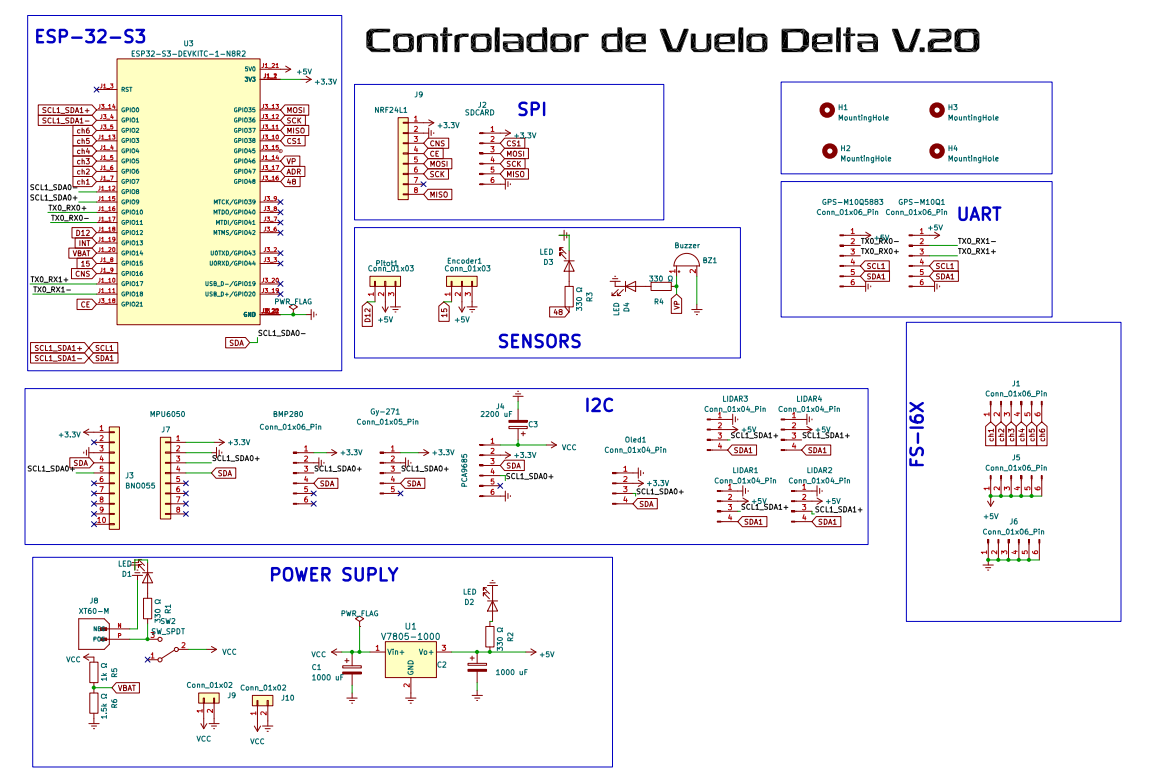
\includegraphics[width=\textwidth]{Imagenes/Metodologia/SCH2.0.png}
    \caption{Esquematico Circuito Impreso 2.0 }
    \label{fig:sch2.0}
\end{figure}

\subsubsection{Diseño del Layout del PCB final} \\ \\

El \textbf{PCB} fue diseñado en dos capas (véase \ref{fig:pcb_2.0} ). En la capa \textbf{TOP} se realizaron varios planos relacionados  con los distintos voltajes de operación del dispositivo, en los que encontramos el de alimentación por batería externa de \textbf{7.4 v}  resaltado en color verde , seguidamente del plano resaltado con color amarillo de \textbf{3.3 v} y finalmente el de \textbf{5v} que serían los planos restantes de \textbf{5V}. En la capa de \textbf{Bottom} se hicieron solamente 2 planos, el de \textbf{7.4 v} resaltado de verde y el de \textbf{GND} que es de color \textbf{azul} en el que se encuentran todas las tierras generales del dispositivo. \\
\begin{figure}[H]
    \centering
    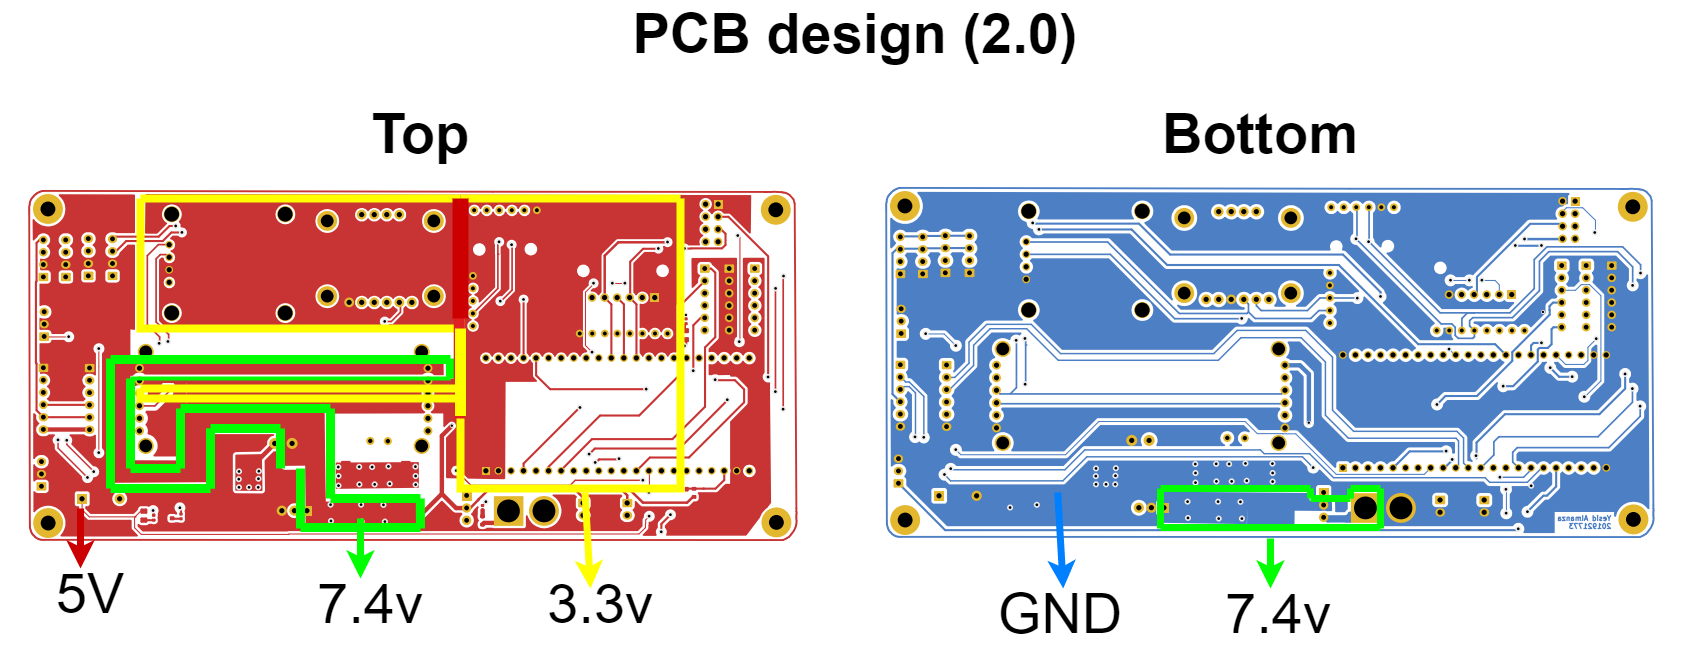
\includegraphics[width=\textwidth]{Imagenes/Metodologia/PCB20.png}
    \caption{Layout Circuito Impreso 2.0 }
    \label{fig:pcb_2.0}
\end{figure}

\\
Para el diseño del layout de la PCB se tuvo en consideración la normativa IPC 2221, la cual establece estándares esenciales para el diseño de placas de circuitos impresos. En la Figura \ref{fig:ipc2221}, se muestran los parámetros clave de esta normativa, incluyendo el ancho de pista, el ancho de separación y la distribución de componentes. Estas directrices aseguran un diseño robusto y seguro, considerando aspectos como la corriente que pueden soportar las pistas, las distancias de separación necesarias según el voltaje, y una distribución eficiente de los componentes para minimizar interferencias y optimizar el rendimiento del circuito.\cite{IPC} \\

\begin{figure}[H]
    \centering
    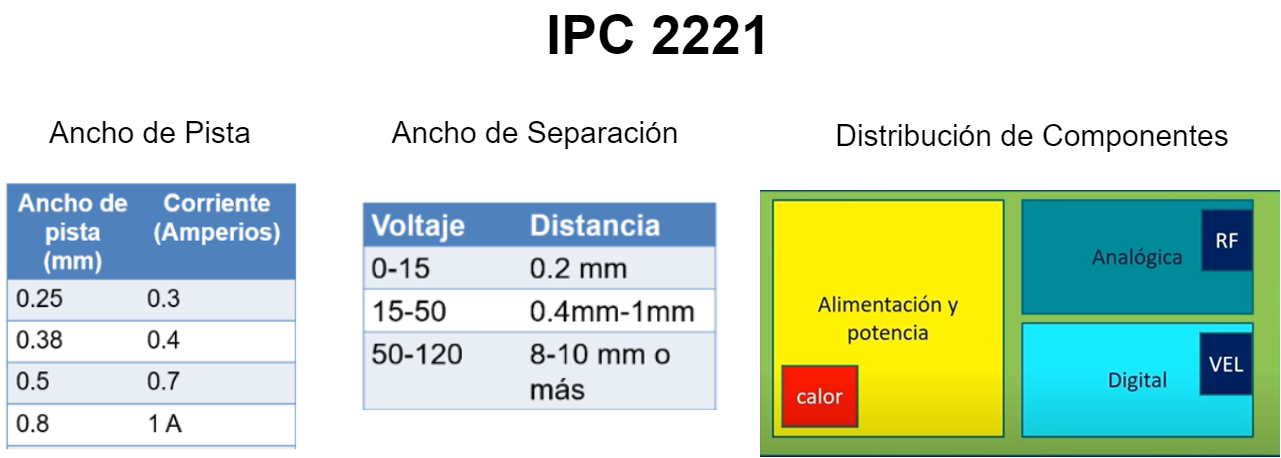
\includegraphics[width=\textwidth]{Imagenes/Metodologia/ipc2221.png}
    \caption{Normativa IPC 2221 \cite{IPC} }
    \label{fig:ipc2221}
\end{figure}

\\
Una vez finalizado el apartado de diseño del layout se procedió a buscar los distintos modelos 3d de los distintos componentes para poder situarlos en un ensamble y observar las dimensiones finales del circuito impreso con los distintos módulos. El tamaño final del \textbf{pcb} fue de \textbf{71.5 mm} de ancho, \textbf{156 mm} de largo \textbf{21.6 mm} de alto. La distribución de los componentes se puede ver a continuación. 
\begin{figure}[H]
    \centering
    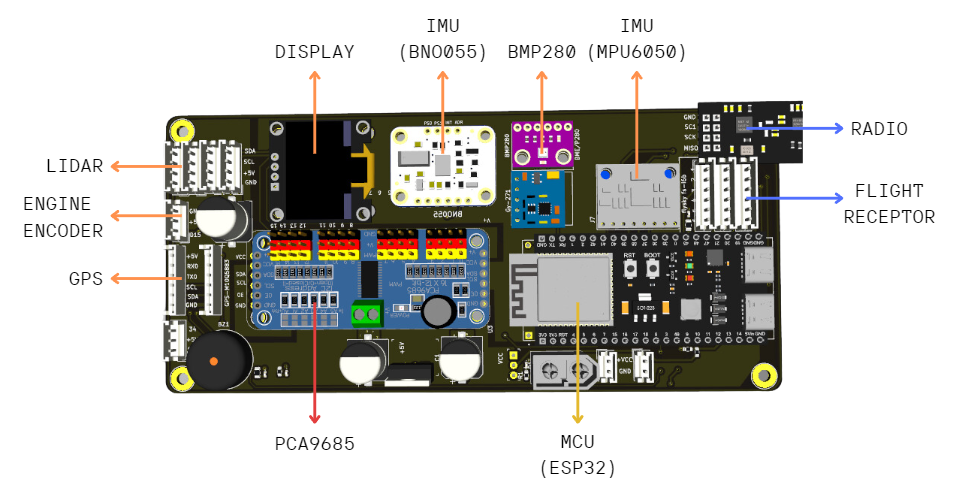
\includegraphics[width=\textwidth]{Imagenes/Metodologia/model3d.png}
    \caption{Modelo 3d Circuito Impreso}
    \label{fig:model3d_pcb}
\end{figure}

\\ \\
\subsubsection{Fabricación del PCB}
\\ \\
El \textbf{Printed Circuit Board (PCB)} fue fabricado en el laboratorio de circuitos impresos de la Universidad de los Andes. Se fabricaron tres de los mismos circuitos en caso de que hubiera algún fallo con alguno de los PCBs. Estos PCBs se fabricaron usando un sustrato de FR4, conocido por su excelente estabilidad térmica y propiedades dieléctricas. Además, el PCB cuenta con tecnología True Hole, lo que garantiza la continuidad eléctrica entre capas.

\\
Para asegurar la calidad y fiabilidad, la fabricación siguió el estándar IPC de fabricación de circuitos impresos, garantizando que el PCB cumple con los requisitos estándares de calidad y rendimiento.
\\

\subsubsection{ Montaje del PCB}
\\ \\

La PCB fue ensamblada teniendo en cuenta los grupos de componentes en ambas capas. Todos los módulos están en la capa superior a excepción del módulo de lectura SD que se encuentra en la capa inferior. Se tomó esta decisión en particular para ahorrar espacio y mejorar la accesibilidad a los componentes significativos durante el mantenimiento y el ensamblaje.

\\ \\

La mayoría de los módulos fueron conectados a través de regletas de inserción, para que en caso de fallo o actualización, los componentes respectivos puedan ser reemplazados sin esfuerzo. Sin embargo, en el módulo SD de lectura, las regletas de inserción no fueron preferidas, ya que estas pueden causar una mala unión mecánica que lleva a la inestabilidad del sistema. La Figura \ref{fig:ensamblada} es una imagen de la tarjeta ensamblada, de la que se puede ver claramente la disposición de los diferentes módulos en la tarjeta. La disposición se ha planeado de tal manera que proporciona un ensamblaje fuerte y adecuado con respecto a las necesidades funcionales y de mantenimiento del equipo.

\begin{figure}[H]
    \centering
    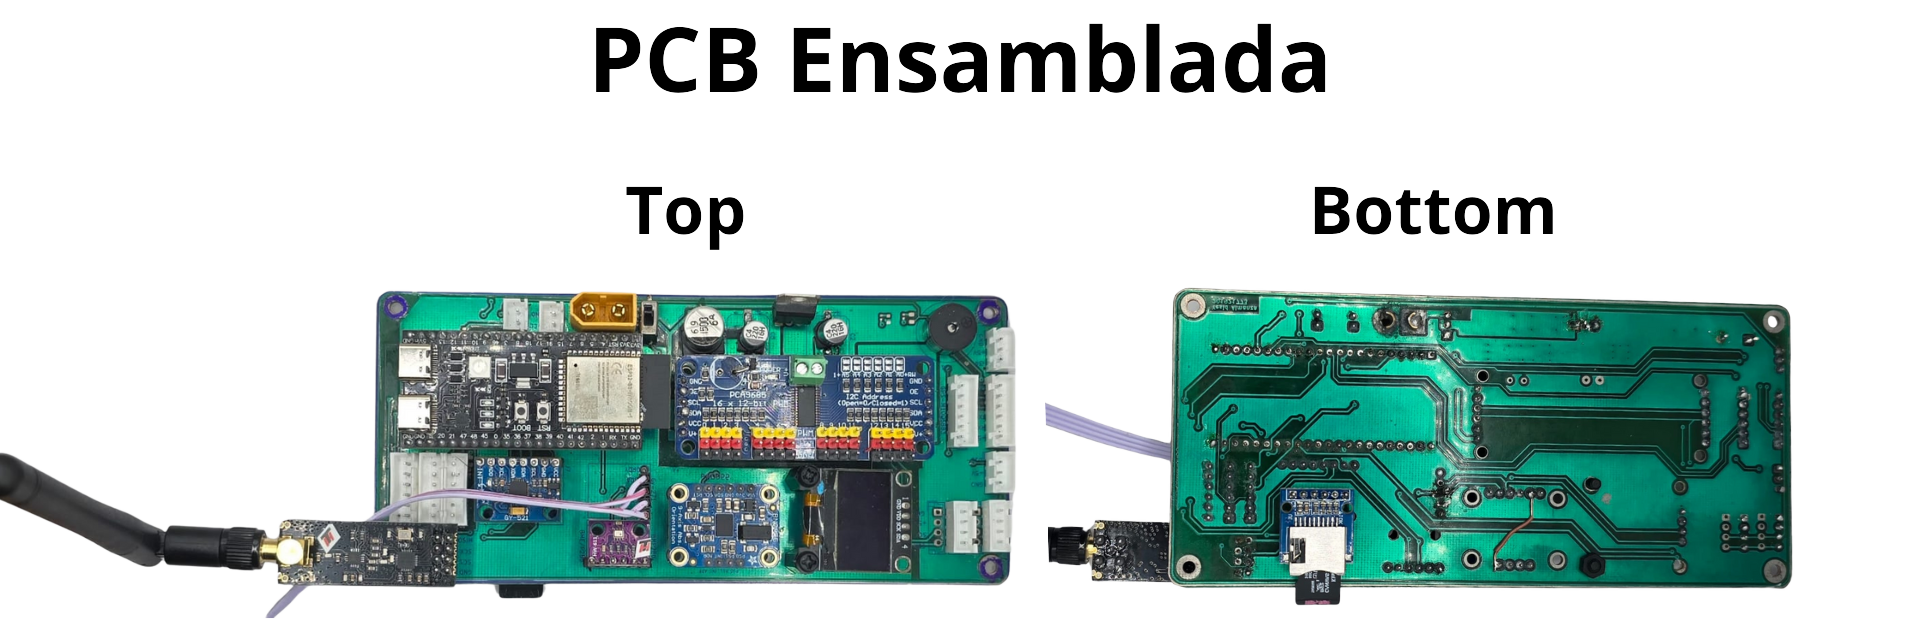
\includegraphics[width=\textwidth]{Imagenes/Metodologia/pcb_ensamblada.png}
    \caption{PCB ensamblada}
    \label{fig:ensamblada}
\end{figure}
\vspace{5 px}\\ \\